%!TEX root = templateICI.tex
%!TEX spellcheck=es_ES

\chapter{Definición del Problema y Análisis}

\section{Formulación del Problema}

Actualmente la empresa Azalée cuenta con un prototipo para la medición de la porosidad y espesor oseo, este prototipo usa la técnica de transmisión axial para realizar las mediciones.
Esta es una técnica desarrollada para medir la propagación de ondas guiadas de ultrasonido en la capa cortical a lo largo del eje de huesos largos.
Los modos guiados propagados en la corteza son grabados con un arreglo de
transductor lineal de 1-MHz.
La medida de la curva de dispersión es obtenida usando una transformada de
fourier de dos dimensiones (espacio, tiempo) combinada con una descomposición
de valores singulares.
La identificación automática de parámetros es obtenida a través de la solución del problema inverso en donde las curvas de dispersión son predichas con un modelo de placa libre isotrópica transversal bidimensional.
La implementación actual de la interfaz humano-computador del prototipo tiene
tiempos de respuesta mayor al deseado.
El prototipo de medición de hueso cortical se muestra en la Figura \ref{fig:hmem}.

\begin{figure}[H]
    \centering
    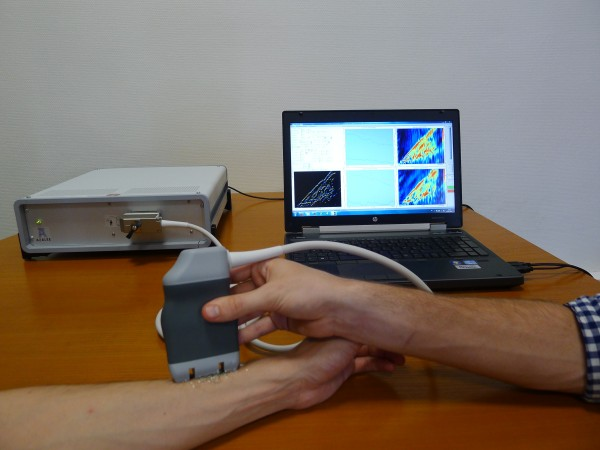
\includegraphics[width=0.75\textwidth]{imagenes/image9.jpg}
    \caption{Prototipo de Azalée.}
    \label{fig:hmem}
\end{figure}




\section{Solución Propuesta}

La solución propuesta al problema consiste en revisar las etapas del algoritmo, modificar el código para reducir complejidades temporales.
Analizar el rendimiento del software implementado para detectar los puntos problemáticos y las áreas dónde sea posible llevar a cabo una optimización del rendimiento.

\section{Objetivos}
A continuación se detallan los objetivos generales y específicos del trabajo de título

\subsection{Objetivo General}
\label{sc:OG}
Disminuir el tiempo de respuesta de la interfaz humano-computador del prototipo
de mediciones corticales de huesos, optimizando las etapas del algoritmo.


\subsection{Objetivos Específicos}
\label{ssc:OE}
\begin{enumerate}
	\item Reducir complejidades temporales del algoritmo de análisis de datos.
	\item Analizar el rendimiento del software implementado (profiling).
	\item Paralelizar código a nivel de datos y tareas.
	\item Acelerar el acceso a memoria ordenando los datos para tomar ventaja del cache del CPU.
    \item Implementar grafico de espesor/porosidad de hueso cortical mediante la resolución del problema inverso.
\end{enumerate}



\section{Metodología}
\label{sc:Met}

La metodología a usar es una cascada ad hoc al problema con una fase iterativa al final.
Esta metodología la componen las siguientes fases.
\begin{enumerate}
    \item \textbf{Aprendizaje}: Fase donde se familiarizara con los principios de la transmisión axial.
    \item \textbf{Analizar Código:} Acá el código y el algoritmo serán analizados.
    \item \textbf{Organizar Modificaciones:} Fase en la cual las modificaciones se ordenaran según las estimaciones de mejoras en el tiempo de respuesta.
    \item \textbf{Realizar modificaciones} Implementación de las modificación.
    \item \textbf{Medir} Etapas donde se prueba la modificación anteriormente realizada.
    \item Si quedan modificaciones por realizar continuar con la siguiente modificación.
\end{enumerate}


En la Figura \ref{fig:met}, se presenta un diagrama de la metodología propuesta.

\begin{figure}[H]
    \centering
    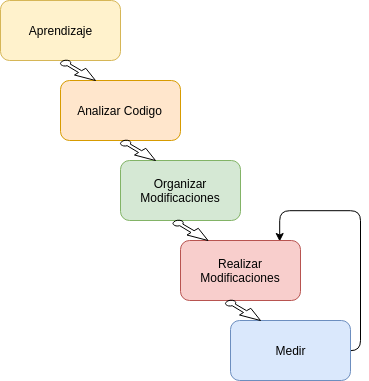
\includegraphics[width=0.75\textwidth]{imagenes/metod.png}
    \caption{Metodología a utilizar}
    \label{fig:met}
\end{figure}

\section{Especificación de Requerimientos}
\label{sc:ER}

A continuación, se detallaran los requisitos funcionales y requisitos no funcionales que el sistema de medición de hueso cortical debe cumplir.
Los requisito funcionales se entienden como una sentencia que identifica lo que el sistema debe cumplir para producir el resultado requerido deseado\cite{adams2015non}.
Los requisitos no funcionales son un requisito del software que no describe lo que el software hará, sino \emph{como} el software lo hará\cite{adams2015non}.

\subsection{Requerimientos Funcionales}
\label{ssc:RF}

En esta sección se detallan los requisitos funcionales del sistema. La sigla   \textbf{RFxx} sera usada en el documento para hacer referencia al requisito funcional.

\begin{itemize}
    \item \textbf{RF01} El sistema mostrara las graficas de espacio de Fourier de las señales recibidas por la sonda de ultrasonido.
    \item \textbf{RF02} El sistema mostrara las graficas de espesor/porosidad del hueso cortical que se este midiendo.
\end{itemize}

\subsection{Requerimientos No Funcionales}
\label{ssc:RNF}

En esta sección se detallan los requisitos no funcionales del sistema. La sigla \textbf{RNFxx} sera usada en el documento para hacer referencia al requisito no funcional.

\begin{itemize}
    \item \textbf{RNF01} El sistema mostrará las gráficas de espacio de Fourier con una frecuencia de al menos cuatro gráficos por segundo.
    \item \textbf{RNF02} El sistema mostrará las gráficas de espesor/porosidad del hueso cortical con una frecuencia de al menos cuatro gráficos por segundo.
    \item \textbf{RNF03} El sistema sera desarrollado usando el lenguaje de programación C++.
\end{itemize}

\section{Funcionalidades del Sistema}
\label{sc:FS}

\subsection{Diagramas de Casos de Uso}
\label{ssc:DCU}

El diagrama de caso de uso representa la interacción del usuario con el sistema que muestra la relación entre el usuario y los diferentes caso de uso en donde el usuario esta involucrado. En el caso del sistema de medición de hueso cortical, en la Figura \ref{fig:dcu} se muestra el único caso de uso que es realizar medición.

\begin{figure}[H]
    \centering
    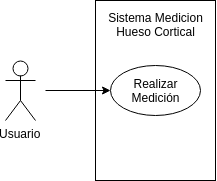
\includegraphics[width=0.75\textwidth]{imagenes/diagrama-caso-usos.png}
    \caption{Diagrama de Caso de Uso del sistema.}
    \label{fig:dcu}
\end{figure}

\subsection{Casos de Uso}
\label{ssc:CU}

% Please add the following required packages to your document preamble:
% \usepackage[normalem]{ulem}
% \useunder{\uline}{\ul}{}

En la siguiente sub-sección se presenta tabla de Caso de Uso extendido.


\begin{table}[H]
\begin{tabular}{ll}


\hline
Nombre:                     & Realizar Medición \\ \hline
Descripción:                & Permite al usuario realizar mediciones\\ &de espesor
y porosidad del hueso cortical  \\ \hline
Actores:                    & Usuario           \\ \hline
Precondiciones:             & Ninguna           \\ \hline
Requisitos No Funcionales: & RNF01,RNF02            \\ \hline
Flujo de Eventos      & 1. El usuario selecciona Realizar Medición \\
&2. Usuario alinea la sonda con el eje del largo del hueso\\
& hasta que obtiene una solución del problema inversor  \\
& 3. Finalizar medición.              \\ \hline
Post-Condiciones            & Ninguna           \\ \hline
\end{tabular}
\end{table}




\subsection{Diagramas de Secuencia}
\label{ssc:DSS}

\subsection{Diagramas de Estado}
\label{ssc:DE}


\subsection{Modelo Conceptual}
\label{ssc:MC}
